\documentclass[long, final]{jobim2017}
% Available options are:
% - showframe 
% - draft
% - final [default]

\usepackage[utf8]{inputenc}
\usepackage{tikz}
\usetikzlibrary{arrows}
\usetikzlibrary{patterns}
\usetikzlibrary{decorations.pathreplacing}
\usepackage{multirow}
\usepackage{mathrsfs}
\usepackage{tabularx}
\usepackage{here}
\usetikzlibrary{automata,positioning}




% WARNING: already loaded packages:
% - hyperref
% - times
% - color
% - xspace
% - graphicx
% - fancyhdr
% - fancybox
% - indentfirst
% - geometry
% - babel (options english,francais) :
%   choose the language with \selectlanguage{<language>}


\pagestyle{empty}
\addtolength{\parskip}{0.4\baselineskip}

%% Title of the paper (required)
\title{HG-CoLoR: A new method for the production of synthetic long reads}

%% List of authors (separated by the macro \and).
%% Authors can be followed by \inst{<n>} macro.
%% The <n> parameter of the \inst macro should correspond to the <n>th institution
%% (see macro \institute below).
\author{Pierre \textsc{Morisse} \and Thierry \textsc{Lecroq} \and Arnaud \textsc{Lefebvre}}

%% List of institutions (separated by the macro \and).
\institute{
 Normandie-Université, UNIROUEN, LITIS EA4108, 76821, Mt-St-Aignan, France
}

% email of the corresponding author
\corresponding{pierre.morisse2@univ-rouen.fr}

% Enter the reference of your paper
%\papername{Morisse \textit{et al.} (2016) HG-CoLoR: A new method for the production of synthetic long reads. \textit{Annals of Improbable Research}. \url{http://dx.doi.org/11.0110/0111/111-1110-0001}}

%% Abstract of the paper (required).
\abstract{%
The recent rise of long read sequencing technologies allows the solving of assembly problems for large and complex genomes that were, until then, unsolvable with the use of short read sequencing technologies alone. Despite the fact that they can reach lengths of tens of kbps, these long reads are very noisy, and can reach an error rate as high as 30\%, involving mandatory error correction before using them to efficiently solve assembly problems. However, as the vast majority of these errors are insertions and deletions, classical error correction tools developed for short reads, which mainly focus on substitution errors, are not effective for correcting long reads. Therefore, several new methods specifically designed for long read error correction have recently been developed. In particular, NaS, instead of directly correcting the long reads, proposes to use them as templates in order to produce synthetic long reads from assemblies of related accurate short reads as corrections. Following this idea, we introduce HG-CoLoR (Hybrid Graph for the error Correction of Long Reads), a new tool for the production of synthetic long reads, that gets rid of the need to align the short reads against each other, which is the bottleneck from NaS. Indeed, HG-CoLoR focuses on a seed-and-extend approach based on a hybrid graph built from the short reads. Our experiments show that, while producing comparable results both in terms of length and accuracy of the synthetic long reads, HG-CoLoR is several times faster than NaS, and also yields better assembly results than other state-of-the-art long read hybrid error correction methods. HG-CoLoR is available from \url{https://github.com/pierre-morisse/HG-CoLoR}.}

%% List of keywords of the paper (required).
\keywords{NGS, long reads, correction, assembly}

\begin{document}

\selectlanguage{english}

\maketitle

%\title{HG-CoLoR: A new method for the production of synthetic long reads}

\section{Introduction}
\label{sec:introduction}

Since a few years, long read sequencing technologies are being developed, and allow the solving of assembly problems for large and complex genomes that were, until then, unsolvable with the use of short reads sequencing technologies alone. The two major actors of these long
read sequencing technologies are Pacific Biosciences and Oxford Nanopore, which, with the release of the MinION device, allows a low-cost and easy long read sequencing. \\
\indent However, even though long reads can reach lengths of tens of kbps, they also reach a very high error rate of around 15\% for Pacific Biosciences, and up to 30\% for Oxford Nanopore, the vast majority of these errors being insertions and deletions. Due to this high error rate, correcting these long reads before using them to efficiently solve assembly problems is mandatory. Many methods are available for short read correction, but these methods are not applicable to long reads, on the one hand because of their much higher error rate, and on the other hand, because most of the error correction tools for short reads focus on substitution errors, the dominant error type in Illumina data, whereas insertions and deletions are more common in long reads. \\
\indent Recently, several methods for long read correction have been developed. These methods can be divided into two main categories: either
the long reads are selfcorrected by aligning them against each other (HGAP \cite{Chin2013}, PBcR \cite{Berlin2015}), or either a hybrid strategy is adopted, in which the long reads are corrected with the help of accurate short reads (LSC \cite{Au2012}, proovread \cite{Hackl2014}, CoLoRMap \cite{Haghshenas2016}). de Bruijn graph \cite{deBruijn1946} based methods, where the long reads are mapped on the graph, and erroneous regions corrected by traversing its paths, also started to develop recently, in the hybrid case (LoRDEC \cite{Salmela2014}, Jabba \cite{Miclotte2016}), as well as in the non-hybrid case (LoRMA \cite{Salmela2016}). \\
\indent NaS \cite{Madoui2015}, instead of directly correcting the long reads, uses them as templates to produce synthetic long reads from assemblies of related accurate short reads. The short reads are mapped both on these templates, and against each other, in order to associate a subset of short reads to each template. A synthetic long read is thus obtained and used as the correction of a given template by assembling the subset of short reads associated to it. \\
\indent In this paper, we introduce HG-CoLoR, a new long read hybrid error correction method that combines both the main idea from NaS to produce synthetic long reads, and the use of a graph, in order to get rid of the time consuming step of aligning all the short reads against each other. HG-CoLoR indeed focuses on a seed-and-extend approach where the seeds, which are short reads that align correctly on the long reads, are used as anchor points on a graph that is traversed in order to link them together and to produce the synthetic long reads. This graph, which is simulated with the help of PgSA \cite{Kowalski2015}, is actually a hybrid structure between a de Bruijn graph and an overlap graph \cite{Ehrenfecht2004}, is built from the short reads' $k$-mers, and allows to compute perfect overlaps of variable length between these $k$-mers. \\
\indent Our experiments show that, while producing comparable results both in terms of length and accuracy of the synthetic long reads, HG-CoLoR is several times faster than NaS, and also yields better assembly results than other state-of-the-art long read hybrid error correction methods. \\
\indent For the sake of understanding, we first give an overview of NaS, and describe our hybrid graph and the way it is simulated, before introducing HG-CoLoR.

\section{NaS Overview}
\label{sec:NaSO}

NaS is a hybrid method for the error correction of long reads that, unlike other methods, uses long reads as templates rather than directly correcting them. Short reads are mapped both on these templates and against each other in order to gather different subsets of short reads, each related to one given template. Each subset is then assembled and the produced contig is used as the correction of the related template. More precisely, a synthetic long read is produced from a template as follows. \\
\indent First, the short reads are aligned on the template using BLAT \cite{Kent2002} in fast mode, or LAST \cite{Kielbasa2011} in sensitive mode, in order to find seeds, which are short reads that align correctly on the template. Then, once these seeds have been found, all the short reads are aligned against each other, and similar reads, which are reads that share a certain number of non-overlapping $k$-mers with the seeds, are recruited with the help of Commet \cite{Maillet2014}. Finally, the obtained subset of short reads is assembled using Newbler (unpublished), and a contig is produced, and used as the correction of the initial template \\ 
\indent The reads recruitment is the most crucial step of the method, as it allows to retrieve short reads corresponding to low quality
regions of the template. However, this step is also the bottleneck of the whole NaS pipeline, as it is responsible for 70\% of the
total runtime on average. \\
\indent NaS is able to generate synthetic long reads up to 60 kbps, that align entirely on the reference genome and that span repetitive regions. On average, the accuracy of the synthetic long reads produced by NaS reaches 99.75\%, without any significant length drop compared to the input long reads. Moreover, these synthetic long reads also yield highly contiguous assembly results, and thus provide an interesting alternative to classical long read hybrid error correction.

\section{Hybrid graph}
\label{sec:HG}

As previously mentioned, the graph used by HG-CoLoR is a hybrid structure between a de Bruijn graph and an overlap graph. This hybrid graph is simulated with the help of PgSA, which is a data structure that allows the indexing of a set of reads of constant length, in order to answer different queries, for a given string $f$. For place sake, we do not detail how the index is built, the complete list of queries, nor how they are processed. For more details, one can refer to \cite{Kowalski2015}. We simply mention that PgSA supports querying for variable lengths of $f$ without recomputing the index, and that one of the queries returns the positions of all the occurrences of $f$ in the different reads of the set. \\
\indent This way, using PgSA to index a set of reads, and looping over the aforementioned query, allows to compute perfect overlaps of variable length between the reads, thus simulating an overlap graph. In the same fashion, indexing the $k$-mers from a set of reads, and looping over the aforementioned query, fixing the length of the queries strings as $k-1$, allows to compute perfect overlaps of length $k-1$ between the $k$-mers, thus simulating a de Bruijn graph. However, indexing the $k$-mers from a set of reads, and looping over the aforementioned query, of course, also allows to compute perfect overlaps of variable length between the different $k$-mers, thus simulating a hybrid structure between a de Bruijn graph and an overlap graph. To the best of our knowledge, this is the first time such a structure is mentioned. For better understanding, an example of a simple graph is given in \hyperref[HGraph]{Figure \ref*{HGraph}}.

\begin{figure}
	\begin{center}
		\resizebox{.8\textwidth}{!}{
		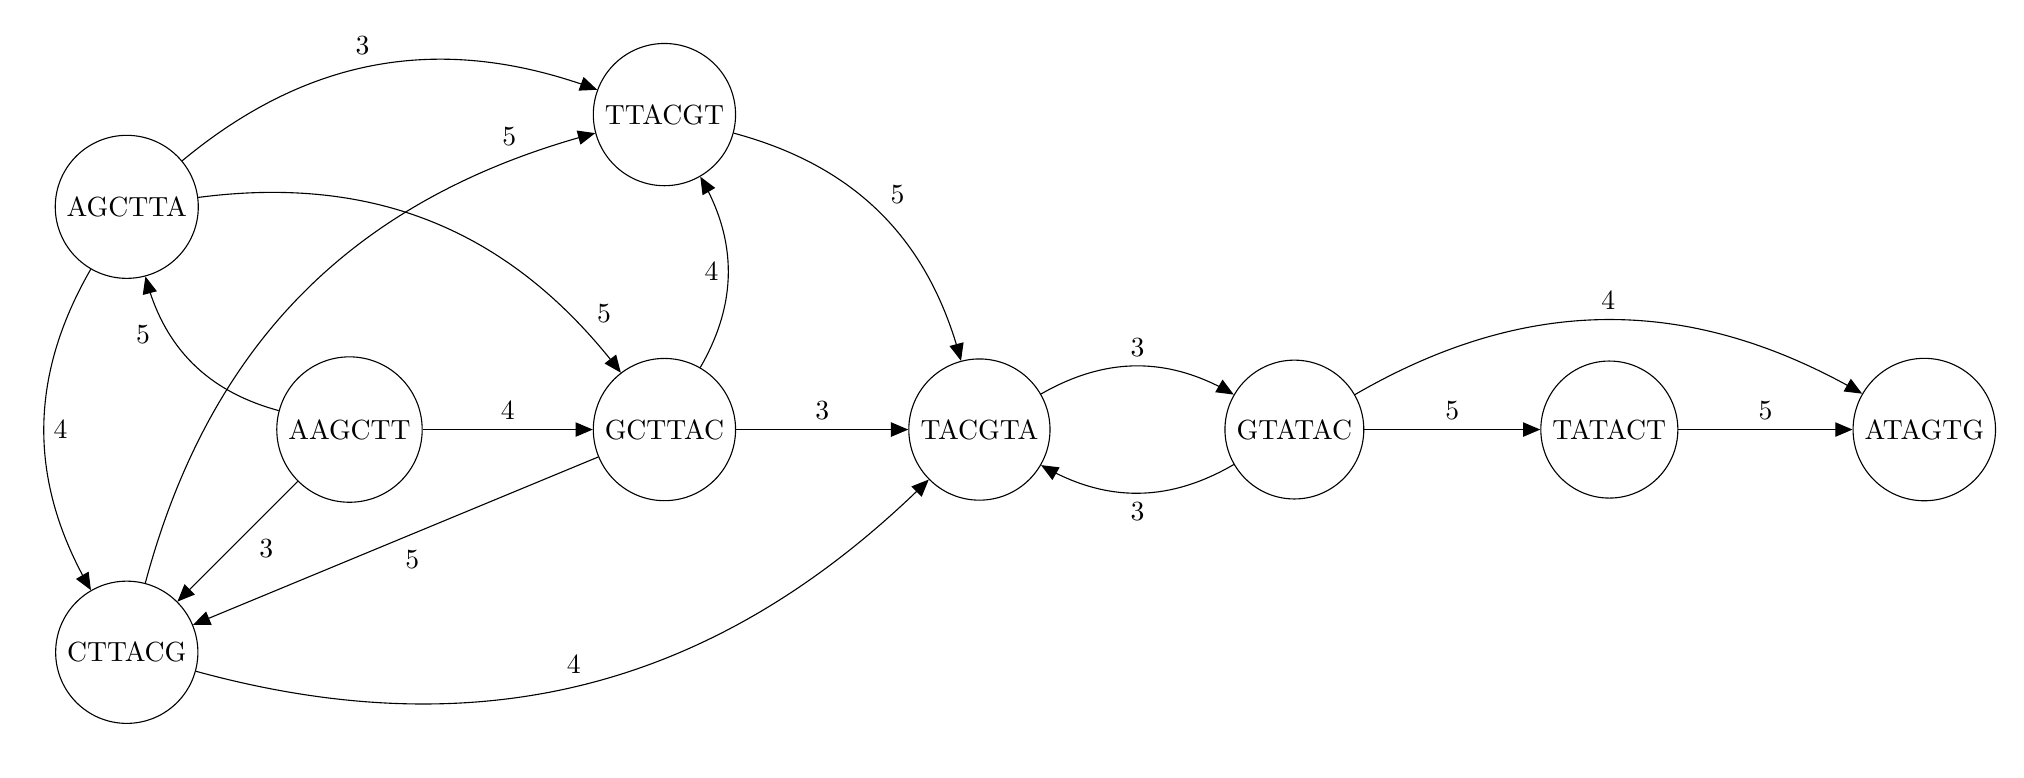
\begin{tikzpicture}[node distance=4cm,auto]
			\node[state] (AAGCTT) {AAGCTT};
			\node[state] [below left of=AAGCTT] (CTTACG) {CTTACG};	
			\node[state] [right of=AAGCTT] (GCTTAC) {GCTTAC};
			\node[state] [right of=GCTTAC] (TACGTA) {TACGTA};
			\node[state] [right of=TACGTA] (GTATAC) {GTATAC};
			\node[state] [right of=GTATAC] (TATACT) {TATACT};
			\node[state] [right of=TATACT] (ATAGTG) {ATAGTG};
			\node[state] [above left of=AAGCTT] (AGCTTA) {AGCTTA};
			\node[state] [above of=GCTTAC] (TTACGT) {TTACGT};
			
			\path[-triangle 45]
			(AAGCTT) edge [bend left] node[pos=0.8] {5} (AGCTTA)
					 edge node {4} (GCTTAC)
					 edge node[pos=.4] {3} (CTTACG)
			(AGCTTA) edge [bend left] node[pos=0.9] {5} (GCTTAC)
					 edge [bend right] node {4} (CTTACG)
					 edge [bend left] node {3} (TTACGT)
			(GCTTAC) edge node {5} (CTTACG)
					 edge [bend right] node {4} (TTACGT)
					 edge node {3} (TACGTA)
			(CTTACG) edge [bend left] node[pos=0.9] {5} (TTACGT)
					 edge [bend right] node {4} (TACGTA)
			(TTACGT) edge [bend left] node {5} (TACGTA)
			(TACGTA) edge [bend left] node {3} (GTATAC)
			(GTATAC) edge [bend left] node {3} (TACGTA)
			(GTATAC) edge node {5} (TATACT)
					 edge [bend left] node {4} (ATAGTG)
			(TATACT) edge node {5} (ATAGTG)
			;
		\end{tikzpicture}
		}
	\end{center}
	\caption{A simple example of our graph, when fixing the length of the $k$-mers to 6, computing overlaps of minimum length 3, and building
	from the three following reads: AAGCTTAC, CTTACGTA, GTATACTG. Numbers on the edges of the graph represent the overlap length 
	between the $k$-mers.
	\label{HGraph}}
\end{figure}

\section{HG-CoLoR description}
\label{sec:OMO}

HG-CoLoR, like NaS, aims to use erroneous long reads as templates, and to produce synthetic long reads from assemblies of short reads related to these templates. However, its main objective is to get rid of the time consuming step of reads recruiting, that requires the mapping of all the short reads against each other. To do so, it focuses on a seed-and-extend approach where the seeds are found in the same way as NaS, and where the $k$-mers from the short reads, and their reverse-complements, are indexed with PgSA, to simulate the previously described graph. This graph is then traversed, in order to extend and link together the seeds, used as anchor points, by directly assembling the short reads' $k$-mers during the traversal. HG-CoLoR's workflow is summarized in \hyperref[OMWorkflow]{Figure \ref*{OMWorkflow}}, and its four main steps are described below.

\begin{figure}
	\begin{center}
	\resizebox{.9\textwidth}{!}{
		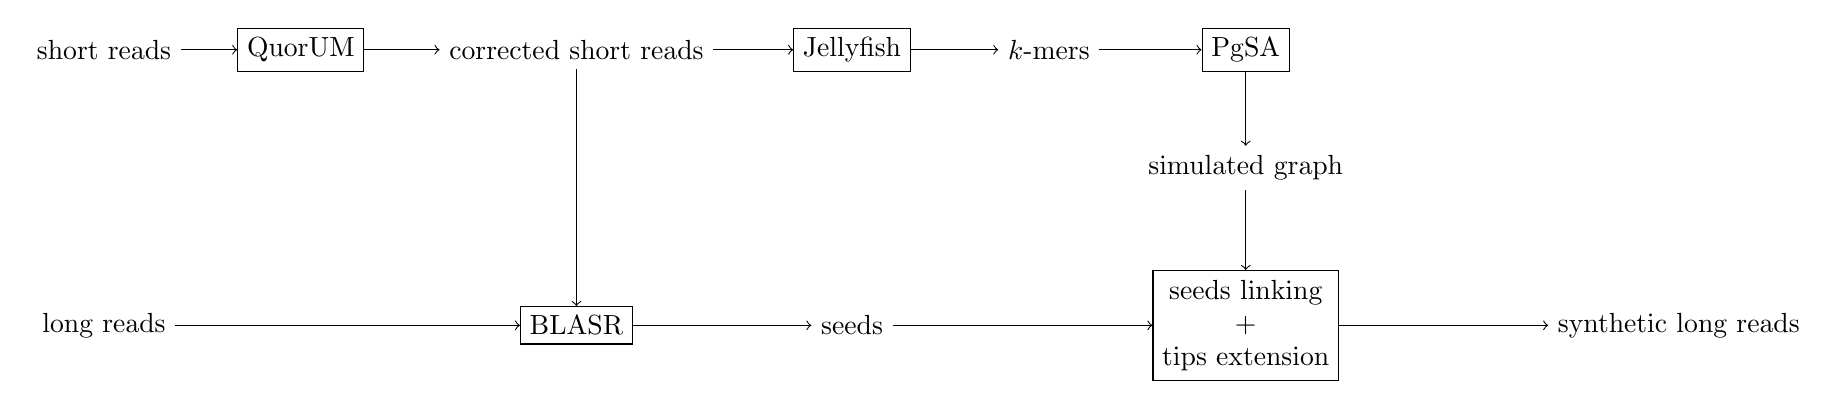
\begin{tikzpicture}			
			\node (SR) at (0,0) {short reads};
			\node[draw, rectangle] (Qu) at (2.5,0) {QuorUM};
			\draw [->] (SR) -- (Qu);
			\node (CSR) at (6,0) {corrected short reads};
			\draw [->] (Qu) -- (CSR);
			\node[draw, rectangle] (Jel) at (9.5,0) {Jellyfish};
			\draw [->] (CSR) -- (Jel);
			\node (kmers) at (12,0) {$k$-mers};
			\draw [->] (Jel) -- (kmers);
			\node[draw, rectangle] (PgSA) at (14.5,0) {PgSA};
			\draw [->] (kmers) -- (PgSA);
			\node (IK) at (14.5,-1.5) {simulated graph};
			\draw [->] (PgSA) -- (IK);			
			\node[draw, rectangle] (BLASR) at (6,-3.5) {BLASR};
			\node (LR) at (0,-3.5) {long reads};
			\draw [->] (LR) -- (BLASR);
			\draw [->] (CSR) -- (BLASR);
			\node (seeds) at (9.5,-3.5) {seeds};
			\draw [->] (BLASR) -- (seeds);
			\node[draw, rectangle, align=center] (Link) at (14.5,-3.5) {seeds linking \\ + \\ tips extension};
			\draw [->] (seeds) -- (Link);
			\draw [->] (IK) -- (Link);
			\node (SLR) at (20,-3.5) {synthetic long reads};
			\draw [->] (Link) -- (SLR);
		\end{tikzpicture}
	}
	\end{center}
	\caption{HG-CoLoR's workflow. First, the short reads are corrected in order to get rid of as much sequencing errors as possible. Then,
	all the $k$-mers from the corrected short reads, and their reverse-complements, are obtained with Jellyfish, and indexed with PgSA, to
	simulate the graph.
	The corrected short reads are aligned on the long reads with BLASR to find seeds, and each long read is then considered as a template, and
	processed
	independently. For a given template, the graph is traversed in order to extend and link together the associated seeds, used as
	anchor points. Then, the tips of the sequence obtained after the seeds linking step are extended in both directions by
	traversing the graph, to reach the
	initial template's borders. Finally, the synthetic long read is output. \label{OMWorkflow}}
\end{figure}

\subsection{Short reads correction and indexing}

Even though short reads are very accurate prior to any correction, as HG-CoLoR seeks to use their $k$-mers to simulate a graph, and traverse it to extend and link the seeds together, it needs to get rid of as much sequencing errors as it can in this data. Thus, prior to any other step, the short reads are corrected with the help of QuorUM \cite{Marcais2015}, which is able to provide a good raise of the accuracy in very little time. Then, the $k$-mers from the corrected short reads, and their reverse-complements, are extracted with Jellyfish \cite{Marcais2011}, and indexed with PgSA, in order to simulate the graph that will be traversed during the following steps.

\subsection{Seeds retrieving and merging}

Like with NaS, the seeds are found by mapping the corrected short reads on the long reads, used as templates. This is done with the help of BLASR \cite{Chaisson2012}, an alignment tool specifically designed to align long reads dominated by insertion and deletion errors. Then, each template is processed independently, and two phases of analyze and merging are applied to the associated seeds. First, if the mapping positions of a given couple of seeds imply that they overlap on the template over a sufficient length, their assumed overlapping sequences are compared, and the two seeds are merged accordingly. If the mapping positions indicate that the two seeds do overlap on the template, but not over a sufficient length, or if the assumed overlapping sequences do not coincide, only the seed with the best alignment score is kept. Then, once all the seeds with overlapping mapping positions have been merged or filtered out, sequence overlaps between consecutive seeds are computed. As in the previous step, if a given seed overlaps the following one over a sufficient length, the two seeds are merged.

\subsection{Seeds linking}

Once the seeds have been found and merged for all of the templates, HG-CoLoR once again processes each template independently and attempts to link the related seeds together by considering them as couples, and traversing the graph. The rightmost $k$-mer of the left seed (source) and the leftmost $k$-mer of the right seed (destination) are used as anchor points, and the source is extended with perfectly overlapping $k$-mers from the corrected short reads, found by following the paths of the graph, until the destination is reached. When facing branching paths, every possible path is explored with the use of backtracking, to find the one that will allow correct linking of the source to destination. Of course, HG-CoLoR explores these different paths in decreasing order of the overlaps lengths, which means that edges representing longer overlaps are always explored before those representing shorter ones. It also only explores edges that represent overlaps that are longer than a defined minimum length. Moreover, as short reads from a different region of the reference genome can align on the template and can be used as seeds, thus leading to impossible linkings, a threshold on the maximum number of backtracks is set, to avoid useless important runtime and intensive computation. \\
\indent If this threshold is reached, and no path has been found to link the source to the destination, the current linking iteration is given up. When such a situation occurs, two different cases have to be taken into account. In the first case, if no seeds have been linked so far, the current source is simply ignored, and a new linking iteration is computed for the next couple of seeds. In the second case, if seeds have already been linked previously, the source remains the same, the destination seed that could not be reached is ignored, and the destination is defined as the next seed for the next linking iteration. An illustration of these two different cases is given in
\hyperref[SeedSkipping]{Figure \ref*{SeedSkipping}}. \\
\indent However, in the second case, as this process of skipping a seed in the middle of the template can provoke an important number of failed linking attempts, if seeds from a wrong region are present in great proportion on the template, a threshold on the maximum number of seeds that can be skipped is set. 
Once this threshold is reached, if the sequence obtained from the previously linked seeds could not be extended to reach one of the remaining seeds, HG-CoLoR attempts to produce a fragmented synthetic long read: the part corresponding to the seeds linked so far is output, and the graph is traversed again, in order to try to link the remaining seeds together, independently of the previous part.

\begin{figure}
\begin{center}
	%TOP
	\resizebox{.9\textwidth}{!}{
	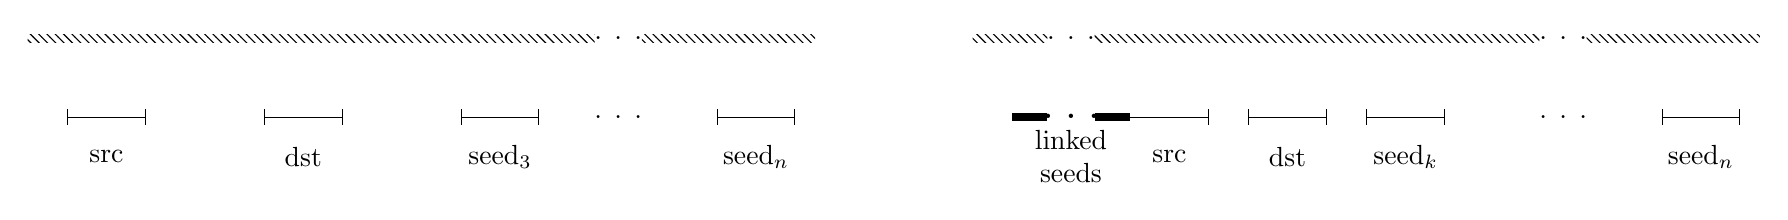
\begin{tikzpicture}
		\fill [pattern=north west lines] (-10,1.05) rectangle (-2.8,0.95);
		\node at (-2.5,1) {. . .};
		\fill [pattern=north west lines] (-2.2,1.05) rectangle (0,0.95);
		\draw [|-|] (-9.5,0) -- (-8.5,0);
		\node at (-9,-0.5) {src};
		\draw [|-|] (-7,0) -- (-6,0);
		\node at (-6.5,-0.5) {dst};
		\draw [|-|] (-4.5,0) -- (-3.5,0);
		\node at (-4,-0.5) {seed$_3$};
		\node at (-2.5,0) {. . .};
		\draw [|-|] (-1.25,0) -- (-0.25,0);
		\node at (-0.75,-0.5) {seed$_n$};
		
		\fill [pattern=north west lines] (2,1.05) rectangle (2.95,0.95);
		\node at (3.25,1) {. . .};
		\fill [pattern=north west lines] (3.55,1.05) rectangle (9.2,0.95);
		\node at (9.5,1) {. . .};
		\fill [pattern=north west lines] (9.8,1.05) rectangle (12,0.95);
		\fill (2.5,-0.05) rectangle (2.95,0.05);
		\node at (3.25,0.005) {\textbf{. . .}};
		\fill (3.55,-0.05) rectangle (4,0.05);
		\node[align=center] (Name) at (3.25,-0.5) {linked \\ seeds};
		\draw [-|] (4,0) -- (5,0);
		\node at (4.5,-0.5) {src};
		\draw [|-|] (5.5,0) -- (6.5,0);
		\node at (6,-0.5) {dst};
		\draw [|-|] (7,0) -- (8,0);
		\node at (7.5,-0.5) {seed$_k$};
		\node at (9.5,0) {. . .};
		\draw [|-|] (10.75,0) -- (11.75,0);
		\node at (11.25,-0.5) {seed$_n$};
	\end{tikzpicture}
	}
	
	%BOTTOM
	\resizebox{.9\textwidth}{!}{
	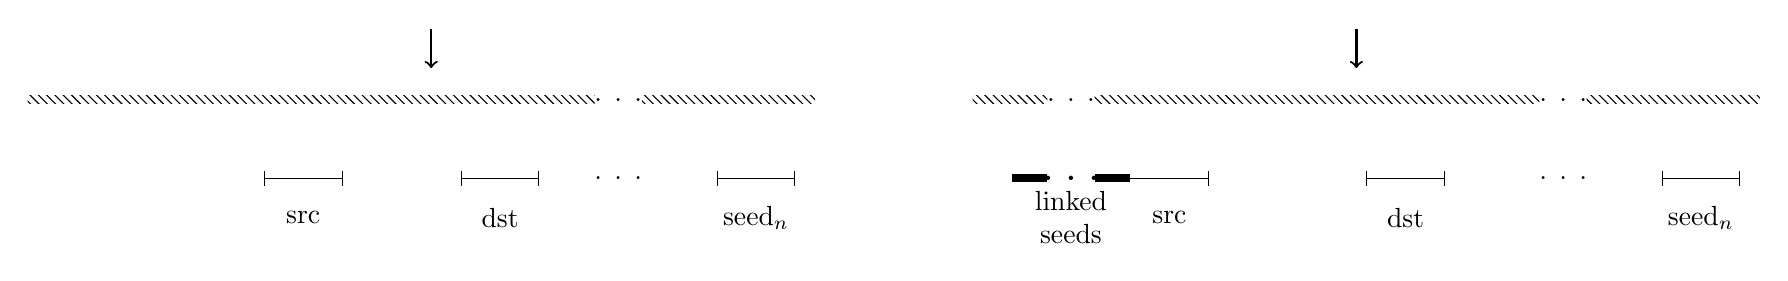
\begin{tikzpicture}
		\draw [->, thick] (-4.875,1.9) -- (-4.875,1.4);
		
		\fill [pattern=north west lines] (-10,1.05) rectangle (-2.8,0.95);
		\node at (-2.5,1) {. . .};
		\fill [pattern=north west lines] (-2.2,1.05) rectangle (0,0.95);
		\draw [|-|] (-7,0) -- (-6,0);
		\node at (-6.5,-0.5) {src};
		\draw [|-|] (-4.5,0) -- (-3.5,0);
		\node at (-4,-0.5) {dst};
		\node at (-2.5,0) {.   .   .};
		\draw [|-|] (-1.25,0) -- (-0.25,0);
		\node at (-0.75,-0.5) {seed$_n$};
		
		\draw [->, thick] (6.875,1.9) -- (6.875,1.4);
		
		\fill [pattern=north west lines] (2,1.05) rectangle (2.95,0.95);
		\node at (3.25,1) {. . .};
		\fill [pattern=north west lines] (3.55,1.05) rectangle (9.2,0.95);
		\node at (9.5,1) {. . .};
		\fill [pattern=north west lines] (9.8,1.05) rectangle (12,0.95);
		\fill (2.5,-0.05) rectangle (2.95,0.05);
		\node at (3.25,0.005) {\textbf{. . .}};
		\fill (3.55,-0.05) rectangle (4,0.05);
		\node[align=center] (Name) at (3.25,-0.5) {linked \\ seeds};
		\draw [-|] (4,0) -- (5,0);
		\node at (4.5,-0.5) {src};
		\draw [|-|] (7,0) -- (8,0);
		\node at (7.5,-0.5) {dst};
		\node at (9.5,0) {. . .};
		\draw [|-|] (10.75,0) -- (11.75,0);
		\node at (11.25,-0.5) {seed$_n$};
	\end{tikzpicture}
	}
\end{center}
\caption{Illustration of the different cases of seed skips. Hatched lines represent the templates, standard segments represent
the seeds, and bold segments represent the sequences obtained from the previously linked seeds. First case (left): No seeds have been linked so far, the current source seed is simply ignored, and both the source and the destination are moved to the next couple of seeds. Second case (right): Seeds have already been linked previously, the source remains the same, the destination seed that could not be reached is ignored, and the destination is defined as the next seed. \label{SeedSkipping}}
\end{figure}

\subsection{Tips extension}

Finally, it is obvious that the seeds do not always map right at the beginning and until the end of the templates. Thus, in order to get as close as possible to the original templates' lengths, once all the seeds of a given template have been linked, HG-CoLoR keeps on traversing the graph and extending the tips of the produced synthetic long read, on the left of the leftmost seed, and on the right of the rightmost seed, until they reach the template's borders, or a branching path. Indeed, in the case of tips extension, when facing a branching path, HG-CoLoR has no clue as to which path to chose and continue the extension with, nor any anchor points, unlike when it attempts to link two seeds together. Therefore, backtracking is useless and the extension is simply stopped when such a situation occurs. In the case of fragmented synthetic long reads, as HG-CoLoR can not properly rely on the template's borders, every fragment is extended until a branching path is reached.

\section{Results and discussion}
\label{sec:results}

We compare the quality of our synthetic long reads with those produced by NaS, and also with the corrected long reads produced by two other state-of-the-art hybrid error correction methods, namely CoLoRMap and Jabba. We compare the results both in terms of alignment identity of the corrected reads, and in terms of quality of the assemblies that could be generated from these reads.

\subsection{Parameters}

We ran multiple rounds of correction with HG-CoLoR on the different datasets to experiment with the parameters, and find the combination that would produce the best results. Thereby, we found that a $k$-mer value of 64 for the graph construction yielded the best compromise between identity, genome coverage, and average length of the output synthetic long reads. The minimum overlap length to allow the merging of two seeds during the second step was set to 63, accordingly to the $k$-mer size chosen for the graph construction. The minimum overlap length allowed to explore an edge during the graph traversal was set to 59, as decreasing it more yielded unsatisfying results, and increasing it would make our graph closer to an actual de Bruijn graph than to the hybrid graph it's supposed to be. The maximum number of backtracks was set to 1,125, as decreasing it more drastically impacted the quality of the produced synthetic long reads, and increasing it, even to very large values, barely yielded better results, but greatly increased the runtime. For the same reason, the maximum number of seed skips was set to 5. For the mapping of the short reads on the long reads, BLASR was used with default parameters except for bestn, that was set to 30 instead of 10. Yet again, increasing this parameter to larger values only impacted the runtime, and did not improve the correction results enough to be interesting, while decreasing it induced a drop of the number of output synthetic long reads. Finally, GNU Parallel \cite{Tange2011} was used to allow HG-CoLoR to run on multiple processes. CoLoRMap was run with default parameters. Following the authors' recommendations, before running Jabba, the short reads were corrected with Karect \cite{Allam2015}, and the de Bruijn graph was constructed and corrected with Brownie (unpublished). A $k$-mer size of 75 was then chosen for the graph construction. All tools were run with 16 processes.

\subsection{Datasets}

As we mainly seek to compare our results with NaS, we use the same data to allow a better comparison. This data is composed of both long Oxford Nanopore reads and short Illumina reads for three different genomes: \emph{Acinetobacter baylyi}, \emph{Escherichia coli}, and \emph{Saccharomyces cerevisae}. Details are given in
\hyperref[tabdata]{Table \ref*{tabdata}}.

\begin{table}[ht]
	\begin{center}
	\resizebox{\textwidth}{!}{
	\begin{tabular}{|c|cccc|ccc|ccc|}
		\hline
		\multirow{2}{*}{\textbf{Dataset}} & \multicolumn{4}{c|}{\textbf{Reference genome}} & 
		\multicolumn{3}{c|}{\textbf{Oxford Nanopore data}} & \multicolumn{3}{c|}{\textbf{Illumina data}} \\
		& \textbf{Name} & \textbf{Strain} & \textbf{Reference sequence} & \textbf{Genome size} & \textbf{\# Reads}
		& \textbf{Average length} & \textbf{Coverage} & \textbf{\# Reads} & \textbf{Read length} 
		& \textbf{Coverage}\\
 		\hline
		\emph{A. baylyi} & \emph{A. baylyi} & ADP1 & CR543861 & 3.6 Mbp & 89,011 & 4,284 & 44x & 900,000 & 250 & 50x \\
		\hline
		\emph{E. coli} & \emph{E. coli} & K-12 substr. MG1655 & NC\_000913 & 4.6 Mbp & 22,270 & 5,999 & 28x & 775,500 & 300 & 50x \\
		\hline
		Yeast & \emph{S. cerevisae} & W303 & scf7180000000084-113 & 12.4 Mbp & 205,923 & 5,698 & 31x & 2,500,000 & 250 & 50x \\
		\hline
	\end{tabular}
	}
	\end{center}
	\caption{Description of the datasets used in our experiments. \label{tabdata} Both MinION and Illumina data are
	available from the Genoscope's website \url{http://www.genoscope.cns.fr/externe/nas/datasets.html}.}
\end{table}

\subsection{Alignment-based comparison}

The previously described long reads datasets were aligned with Last prior to any correction. The four different correction tools were then applied, and the obtained corrected long reads were aligned with BWA mem \cite{Li2010b}. Results are given in \hyperref[tabid]{Table \ref*{tabid}} and discussed below.

\begin{table}[ht]
	\begin{center}
	\resizebox{\textwidth}{!}{
	\begin{tabular}{|c|c|c|c|c|c|c|c|c|c|}
		\hline
		\textbf{Dataset} & \textbf{Method} & \textbf{\# Reads} & \textbf{Average length} & \textbf{Cumulatize size}
		& \textbf{\# Aligned reads} & \textbf{Average identity} & \textbf{\# Error-free reads} 
		& \textbf{Genome coverage}
		& \textbf{Runtime} \\
		\hline		
		\multirow{6}{*}{\emph{A. baylyi}} & Original & 89,011 & 4,284 & 381,365,755 & 29,954 (33.65\%) & 70.09\% & 0 (0\%) & 100\% & N.A. \\
		& CoLoRMap & 89,011 & 4,355 & 387,609,994 & 18,085 (20.32\%) & 67.93\% & 2 (0.01\%) & 100\% & 14h33min \\
		& Jabba & 17,476 & 10,260 & 179,309,738 & 17,476 (100\%) & 99.40\% & 16,893 (96.66\%) & 99.80\% & 12min30 \\
		& NaS (fast) & 24,063 & 8,840 & 212,707,189 & 24,063 (100\%) & 99.82\% & 22,984 (95.52\%) & 100\% & \_ \\
		& NaS (sensitive) & 28,492 & 9,530 & 271,526,778 & 28,492 (100\%) & 99.83\% & 27,190 (95.43\%) & 100\% & \_ \\
		& HG-CoLoR & 23,465 & 11,137 & 261,327,970 & 23,461 (99.98\%) & 99.44\% & 20,906 (89.11\%) & 100 \% & 21h08min \\
		\hline
		\multirow{6}{*}{\emph{E. coli}} & Original & 22,270 & 5,999 & 133,607,392 & 22,170 (99.55\%) & 79.46\% & 0 (0\%) & 100\% & N.A. \\
		& CoLoRMap & 22,270 & 6,219 & 138,489,144 & 21,784 (97.82\%) & 89.02\% & 152 (0.70\%) & 100\% & 8h26min \\
		& Jabba & 22,065 & 5,794 & 127,848,525 & 22,065 (100\%) & 99.81\% & 21,850 (99.03\%) & 99.41\% & 12min56 \\
		& NaS (fast) & 21,818 & 7,926 & 172,918,739 & 21,818 (100\%) & 99.86\% & 20,383 (93.42\%) & 100\% & \_ \\
		& NaS (sensitive) & 22,144 & 8,307 & 183,958,832 & 22,144 (100\%) & 99.86\% & 20,627 (93.15\%) & 100\% & \_ \\
		& HG-CoLoR & 22,549 & 5,897 & 132,979,813 & 22,549 (100\%) & 99.59\% & 19,676 (87.26\%) & 100\% & 15h15min \\
		\hline
		\multirow{6}{*}{Yeast} & Original & 205,923 & 5,698 & 1,173,389,509 & 68,215 (33.13\%) & 55.49\% & 0 (0\%) & 99.90\% & N.A. \\
		& CoLoRMap & 205,923 & 5,737 & 1,181,298,941 & 40,530 (19.68\%) & 39.93\% & 23 (0.06\%) & 99.40\% & 37h36min \\
		& Jabba & 36,958 & 6,613 & 244,402,749 & 36,855 (99.72\%) & 99.55\% & 34,028 (92.33\%) & 93.21\% & 44min05 \\
		& NaS (fast) & 71,793 & 5,938 & 426,326,355 & 71,664 (99.82\%) & 99.59\% & 59,788 (83.43\%) & 98.70\% & \_ \\
		& NaS (sensitive) & 85,432 & 6,770 & 578,351,588 & 85,288 (99.83\%) & 99.53\% & 69,816 (81.86\%) & 99.17\% & \_ \\
		& HG-CoLoR & 71,284 & 6,576 & 468,735,999 & 71,161 (99.83\%) & 99.18\% & 55,240 (77.63\%) & 98.39\% & 112h20min \\
		\hline
	\end{tabular}
	}
	\end{center}
	\caption{Runtime and statistics of the long reads, before and after correction by the different tools. 
	NaS runtimes are omitted because results did not compute in 3 days, even for \emph{E. coli} in fast mode. NaS reads 
	were therefore obtained from the Genoscope's website to allow comparison.
	\label{tabid}}
	
\end{table}

We notice that, unlike the other methods, CoLoRMap output all the long reads and not only the ones it managed to correct. As the reads that could be corrected were not tagged in any way and could therefore not be extracted, it appears that CoLoRMap performed the worst correction, and did not manage to improve the accuracy of the long reads at all, except for the \emph{E. coli} dataset. These poor results are probably due to the fact that only a few reads could be corrected, as CoLoRMap is designed to correct long reads from Pacific Biosciences, that have an error rate of about 15\%, whereas the long reads used in our experiments were from Oxford Nanopore, and reached an error of at least 30\% for the two other datasets. \\
\indent Jabba clearly performed the best when it comes to runtime, outperforming all the other tools by several orders of magnitude. It also produced corrected long reads that aligned with a high identity, a great proportion of them aligning with no error. However, although highly accurate, these corrected long reads did not manage to completely cover any of the studied reference genomes. \\
\indent When it comes to this point, only NaS and HG-CoLoR managed to cover the whole reference genomes with high identity, except for Yeast, due to the fact that even the original long reads did not cover the whole genome. This proves that focusing on the production of synthetic long reads is indeed a good alternative to classical long read hybrid error correction. Moreover, HG-CoLoR outperforming Jabba in terms of genome coverage also clearly underlines the usefulness of our hybrid graph, showing that it allows to resolve the different regions of the reference genomes better than a classical de Bruijn graph. \\
\indent On the three datasets, NaS yielded more synthetic long reads than HG-CoLoR, both in fast and sensitive mode, the slight advantage of HG-CoLoR on the \emph{E. coli} dataset coming from the production of fragmented synthetic long reads, rather than from a greater number of processed templates. In both modes, the synthetic long reads produced by NaS also aligned with a slightly higher identity than those produce by HG-CoLoR, and a greater proportion was therefore error-free. As for the average length and the cumulative size of the synthetic long reads, HG-CoLoR performances were highly similar to NaS's, except on the \emph{E.coli} dataset, where the advantage of NaS is probably due to the high quality of the original templates, and to the fact that it can recruit short reads outside of the templates, while HG-CoLoR stops once the borders are reached. However, despite its slight disadvantage on the aforementioned metrics, HG-CoLoR was at least four times faster than NaS, even in fast mode.

\subsection{Assembly-based comparison}
	
All the corrected long reads datasets previously described were assembled using Canu \cite{Koren2016}, without the correction and trimming steps. The following parameters were used for the assembly of all the datasets: OvlMerSize=17, MhapMerSize=17, OvlMerDistinct=0.9925, OvlMerTotal=0.9925. The correctedErrorRate parameter was tuned independently for each dataset. It was set at 0.07 for \emph{A. baylyi}, at 0.085 for \emph{E. coli} and at 0.125 for Yeast. Results are given in \hyperref[tabas]{Table \ref*{tabas}} and discussed below.

\begin{table}[ht]
	\begin{center}
	\begin{tabular}{|c|c|c|c|c|c|c|}
		\hline
		\textbf{Dataset} & \textbf{Method} & \textbf{\# Reads} & \textbf{\# Expected contigs} & \textbf{\# Obtained contigs} & \textbf{Genome coverage} 
		& \textbf{Identity} \\
		\hline
		\multirow{5}{*}{\emph{A. baylyi}} & CoLoRMap & 89,011 & 1 & \_ & \_ & \_ \\
		& Jabba & 17,476 & 1 & 13 & 89.43\% & 99.93\% \\
		& NaS (fast) & 24,063 & 1 & 1 & 100 \% & 99.99 \% \\
		& NaS (sensitive) & 28,492 & 1 & 2 & 99.72\% & 99.98\% \\
		& HG-CoLoR & 23,465 & 1 & 1 & 99.97\% & 99.93\% \\
		\hline
		\multirow{5}{*}{\emph{E. coli}} & CoLoRMap & 22,270 & 1 & 29 & 97,74\% & 99.81\% \\
		& Jabba & 22,065 & 1 & 41 & 95.76\% & 99.92\% \\
		& NaS (fast) & 21,818 & 1 & 1 & 99.90 \% & 99.99\% \\
		& NaS (sensitive) & 22,144 & 1 & 2 & 100\% & 99.99\% \\
		& HG-CoLoR & 22,549 & 1 & 2 & 99.95\% & 99.95\% \\
		\hline
		\multirow{5}{*}{Yeast} & CoLoRMap & 205,923 & 30 & \_ & \_ & \_ \\
		& Jabba & 36,958 & 30 & 134 & 70.52\% & 99.83\% \\
		& NaS (fast) & 71,793 & 30 & 123 & 97.44\% & 99.77\% \\
		& NaS (sensitive) & 85,432 & 30 & 123 & 96.98\% & 99.80\% \\
		& HG-CoLoR & 71,284 & 30 & 109 & 92.76\% & 99.63\% \\
		\hline
	\end{tabular}
	\end{center}
	\caption{Statistics of the assemblies that were generated from the long reads, after correction by the different tools. CoLoRMap results are ommitted 
	for the \emph{A. baylyi} and Yeast datasets, because Canu did not manage to assemble the sets of corrected reads.
	\label{tabas}}
\end{table}

In agreement with what we observed in \hyperref[tabid]{Table \ref*{tabid}}, the low accuracy of the long reads corrected by CoLoRMap resulted in impossible assemblies. Only the corrected long reads of the \emph{E. coli} dataset could be assembled, due to their original high accuracy, but the generated assembly did not cover the whole genome, and displayed the worst identity among all the other assemblies. \\
\indent As for Jabba, the fact that the corrected long reads did not manage to cover the whole reference genomes resulted in highly fragmented assemblies, that could not resolve large regions of the reference genomes. As a result, long reads corrected by Jabba yielded the least covering assemblies, despite their high average length and high accuracy. This underlines the fact that, although it is extremely fast, Jabba does not seem to be adapted for correcting long reads prior to an assembly. \\
\indent Surprisingly, for all the datasets, the sensitive mode of NaS produced synthetic long reads that resulted in slightly less satisfying assemblies than the fast mode. However, the difference was not significant, and adapting the parameters of Canu to match the synthetic long reads produced in sensitive mode addressed this issue. \\
\indent Therefore, only the synthetic long reads produced by NaS and HG-CoLoR could be assembled into a decent number of contigs, covering the reference genomes well, and with a high identity. However, for the Yeast dataset, none of these two tools managed to produce synthetic long reads allowing to get close to the expected number of contigs, nor to the full genome coverage. This is probably due to the fact that the original long reads were of really poor quality, displaying an error rate of almost 45\%, and did not cover the whole genome. They were indeed sequenced with an old chemistry, and it is more than likely that, with long reads from a more recent one as templates, both NaS and HG-CoLoR could produce synthetic long reads that would greatly reduce the number of contigs and increase the genome coverage of the assembly. We can also suppose that NaS outperforms HG-CoLoR on this dataset for this very same reason, and that using long reads from a more recent chemistry as templates would allow HG-CoLoR to compare much better to NaS. \\
\indent Once again, these results prove that focusing on the production of synthetic long reads, rather than on the direct correction of the long reads, is a good alternative to classical long read hybrid error correction.

\section{Conclusion}
\label{sec:conclusion}

We described HG-CoLoR, a new hybrid method for the error correction of long reads, that, like NaS, uses long reads as templates and focuses on the production of synthetic long reads, rather than on the direct correction of the input long reads. Our method, instead of aligning the short reads against each other in a recruiting step, like NaS, focuses on a seed-and-extend approach and introduces a brand new idea of using a hybrid structure between a de Bruijn graph and an overlap graph. This graph, which is built from the short reads' $k$-mers, and simulated with PgSA, is used to extend and link together the seeds, which are short reads that align correctly on the input long reads, by a simple traversal, using them as anchor points. Therefore, the synthetic long reads are produced by directly assembling the short reads' $k$-mers during the traversal, without using any other proper assembly tool. \\
\indent We tested this new method and compared it with NaS, CoLoRMap and Jabba on Oxford Nanopore long reads from three different genomes, namely \emph{A. baylyi}, \emph{E. coli}, and \emph{S. cerevisae}. On these three datasets, HG-CoLoR yielded results that compared well with NaS, while being several times faster, CoLoRMap produced corrected reads of poor quality, and Jabba, while being the fastest tool, produced accurate corrected reads that however did not cover the whole reference genomes. As a result, only the synthetic long reads produced by NaS and HG-CoLoR could be assembled into a decent number of contigs, covering well the reference genomes, although NaS outperformed HG-CoLoR on the \emph{S. cerevisae} dataset. \\
\indent The development of this method shows that, when having anchor points, the previously introduced hybrid graph can prove useful for hybrid error correction of long reads, and can even yield better results than a classical de Bruijn graph. For future works, it could be interesting to focus more on this graph, and directly build it instead of simulating it, in order to directly map the long reads on the graph, like Jabba, thus skipping the alignment step of the short reads on the long reads, and reducing the runtime.

\section*{Acknowledgements}

The authors would like to thank the Genoscope team for the availability of all the data used in this paper.

\bibliography{../../../../../Bibliographies/library}
\end{document}
